\documentclass[tikz,border=10pt]{standalone}
\usepackage{fontspec}
\usetikzlibrary{arrows.meta,calc}

\setmainfont{Latin Modern Roman}

\definecolor{navy}{HTML}{163A5F}
\definecolor{amber}{HTML}{A85D00}
\definecolor{teal}{HTML}{157A73}
\definecolor{slate}{HTML}{536878}
\definecolor{lightgray}{HTML}{AAB5BE}

\begin{document}
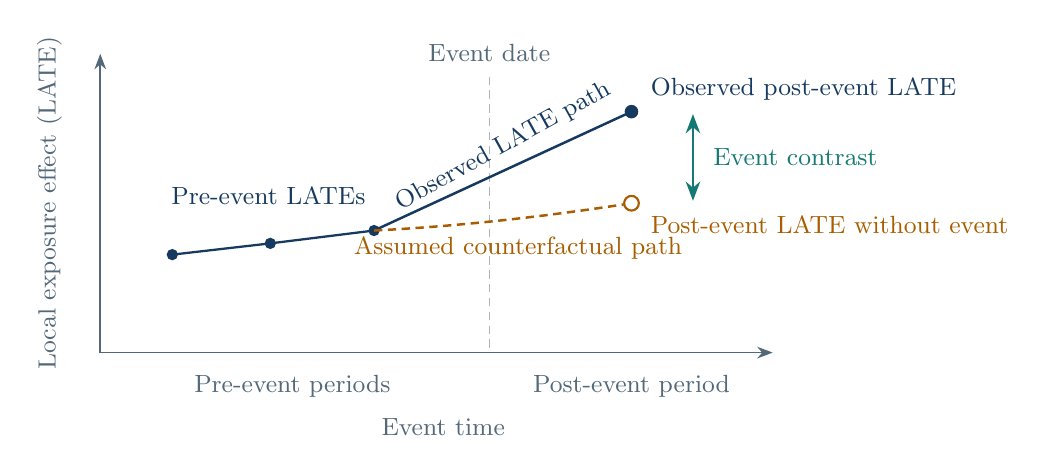
\begin{tikzpicture}[
  x=1.22cm,
  y=1.02cm,
  >={Stealth[length=2.6mm,width=1.8mm]},
  annotation/.style={font=\fontsize{8.6}{10}\selectfont,align=center},
  keylabel/.style={font=\fontsize{9.2}{10.8}\selectfont,align=left}
]

% Axes and event date
\draw[-{Stealth},slate,line width=0.58pt] (-4.05,0) -- (2.95,0);
\draw[-{Stealth},slate,line width=0.58pt] (-4.05,0) -- (-4.05,3.72);
\draw[lightgray,densely dashed,line width=0.58pt] (0,0.06) -- (0,3.48);

\node[annotation,color=slate,anchor=north] at (-2.05,-0.16) {Pre-event periods};
\node[annotation,color=slate,anchor=north] at (1.48,-0.16) {Post-event period};
\node[annotation,color=slate,anchor=south] at (0,3.50) {Event date};
\node[annotation,color=slate,anchor=north] at (-0.48,-0.70) {Event time};
\node[annotation,color=slate,rotate=90] at (-4.58,1.86) {Local exposure effect (LATE)};

% Comparable pre-event LATEs
\draw[navy,line width=0.82pt]
  (-3.30,1.22) -- (-2.28,1.36) -- (-1.20,1.52);
\foreach \x/\y in {-3.30/1.22,-2.28/1.36,-1.20/1.52}{
  \fill[navy] (\x,\y) circle (2.05pt);
}
\node[keylabel,color=navy,anchor=south] at (-2.30,1.72)
  {Pre-event LATEs};

% Observed LATE path
\draw[navy,line width=0.90pt]
  (-1.20,1.52) -- (1.48,3.00);
\fill[navy] (1.48,3.00) circle (2.45pt);
\node[keylabel,color=navy,anchor=south west] at (1.58,3.02)
  {Observed post-event LATE};
\node[annotation,color=navy,rotate=29,anchor=south]
  at (0.25,2.34) {Observed LATE path};

% Assumed counterfactual path
\draw[amber,densely dashed,line width=0.90pt]
  (-1.20,1.52) .. controls (-0.20,1.58) and (0.72,1.72) .. (1.48,1.86);
\draw[amber,line width=0.78pt,fill=white] (1.48,1.86) circle (2.65pt);
\node[annotation,color=amber,anchor=north]
  at (0.30,1.56) {Assumed counterfactual path};
\node[keylabel,color=amber,anchor=north west] at (1.58,1.82)
  {Post-event LATE without event};

% Event contrast at the post-event date
\draw[{Stealth}-{Stealth},teal,line width=0.88pt]
  (2.12,1.89) -- (2.12,2.97);
\node[keylabel,color=teal,anchor=west] at (2.23,2.43)
  {Event contrast};

\end{tikzpicture}
\end{document}
